% !TEX root = mythesis.tex

%==============================================================================
\chapter{Monte Carlo simulation}
\label{sec:MC}
%==============================================================================
The MC simulation for NA64 visible mode for the 2018 setup has been implemented by the collaboration in GEANT4. The information from the MC simulation is currently reconstructed in a standalone reconstruction program similar to how it is done for real data. This chapter tries to document how the simulation is implemented. This is an important facet since the type of process we are trying to study is not part of the SM and is required to be implemented as an extra step to a standard GEANT4 simulation. Though these processes were added in the physics code~\cite{Gninenko:2017yus,PhysRevD.97.072002} it is still important to document how they are included in a simulation.

Since one of the main goals is to implement the data analysis chain in CORAL, reconstructing the MC simulation output (MCTruth) in CORAL is a part of this goal. Thus, the chapter also details the changes made to the MCTruth to make it compatible with CORAL along with the results of the said reconstruction.

\section{$A'$ Production}
$A'$ production in the NA64 simulation has been described in~\cite{Gninenko:2017yus}. A short summary for the procedure is as follows:
\begin{description}
  \item $-$ The emission probability for $A'$ production for an active target which in our case is fixed to be Pb is given as $P_{emission} = \rho N_A \sigma_{tot}^{A'} \Delta L_i / A $ where $\rho$ is the density of the target, $N_A$ is the Avogadro's number, $\sigma_{tot}^{A'}$ is the total cross-section for the $A'$ production in a bremsstrahlung like reaction as mentioned before, $\Delta L_i$ is the step length of the electron path in the target and $A$ is the atomic weight.

  The total cross-section is approximated by using IWW approximation however as it is seen in the fig.(\ref{fig:ETLvsIWW}), ETL calculation is more accurate and complete. The error in the cross-section calculation is fixed by introducing a K-factor defined as $K = \sigma_{IWW}^{A'} / \sigma_{ETL}^{A'}$.

  \item $-$ A sample variable $u_1$ is randomly sampled from a uniform distribution over the unit interval [0,1]. If $u_1$ is found to be smaller than the emission probability $P_{emission}$ the the simulation for $A'$ proceeds further.

  \item $-$ For an $A'$ emission a random picking for the relevant kinetic parameters $x$, $cos\theta$ and the azimuthal angle $\phi$ is done. The simulation for $A'$ emission and decay continues if the parameters are accepted after rejection sampling.

  \item $-$ Next the kinetic energy for the emitted $A'$ is set. Based on this value it is checked whether at the simulated $A'$ mass the dark photon can escape the subsequent WCAL catcher which is directly after the active target for the visible mode. If this is true then the $A'$ is simulated to decay into $e^+e^-$ and the relevant information about $A'$ and the decay particles which include mass, decay position and momentum is recorded.
\end{description}

\begin{figure}[t!]
\centering
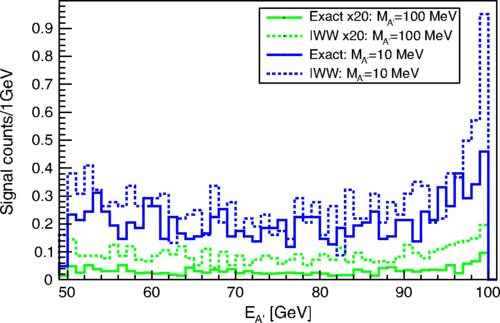
\includegraphics[width=12cm]{thesis_figures/IWWvsETL.png}
\caption{Number of simulated signal events at two $A'$ masses as a function of Dark Photon energy~\cite{Gninenko:2017yus}}
\label{fig:ETLvsIWW}
\end{figure}

\section{Tracking Detectors}
NA64 consists of two sets of tracking detectors namely Micromegas and GEMs. In the visible mode simulation two Micromegas named MM1 and MM2 are placed upstream of the two magnets and two more named MM3 and MM4 are placed right after the vacuum tube and before the WCAL. Four additional GEM detectors are placed right after the downstream WCAL. Both GEMs and Micromegas have the same implemented internal structure in the simulation. The structure consists of an Argon gasbox surrounded by two Mylar layers on either side. An additional layer of Copper and PCB is added after the second Mylar layer. The gas volume is set as sensitive for both Micromegas and GEMs.

While processing the output of the simulation for the tracking detectors the following information about each particle traversing the detector is recorded- x,y and z hit positions, energy deposited, trackID of the particle, the PDG~\cite{pdg2010} encoding of the particle and the kinetic energy. The trackID is a unique ID which GEANT4 gives to each particle simulated and tracked during the simulation. The trajectories and the origin of \emph{all} the simulated and tracked particles are not saved in the current format. Some trajectories such as those of the beam particle and the simulated $A'$ along with its decay products is available. Saving all trajectories should be considered in the future since the information is useful for reconstruction.

To reconstruct the simulation output it was modified to a format that can be read in CORAL described more in appendix(\ref{sec:app_2}). This comprised of including information such as a unique identifier for each tracking detector (Detector name + DetectorID), particle trajectories for relevant simulated particles and splitting the information to individual detector planes for implementation in CORAL. Additional options were provided in the track fitting option files to activate MC decoding. The reconstruction in GEMs proceeds in the following way:
\begin{enumerate}
  \item For an event CORAL reads in the hit positions for the individual detectors and checks the validity of the TrackIDs against provided trajectories.
  \item Next it moves on to the detector response simulation where it uses the hit data along with extra simulation parameters to simulate three amplitudes for each detector. The simulation parameters include space resolution of the detector (mm), effective gain of the detector along with the standard deviation, signal width (mm) and time resolution (ns) if the timing information is available. The simulation parameters are fed through the track option file.
  \item The simulated amplitude is calculated as follows, $ amp = \frac{1}{\sqrt{2\pi}}\frac{(\text{Energy~deposited} \times (\text{Effective gain} + \sigma_{\text{Gain}}))^2}{\text{signal width}} $ with inbuilt cuts to remove meaningless hits.
  \item The simulated amplitude for the hit is then assigned to the nearest readout strips it might corroborate to.
  \item The amplitudes for each strip are then passed to clusterization and tracking.
\end{enumerate}
The reconstruction for the tracking detectors is evaluated by looking at the reconstructed momentum.

\section{Calorimeters}
 As mentioned before, NA64 consists of three types of calorimeters namely WCAL, ECAL and HCAL in the visible mode setup. The WCAL is simulated to consist of three layers similar to the real setup. These are the pre-shower, main and the catcher. After the simulation the total energy deposited in each layer is calculated for each simulated event. The ECAL also has the same structure in GEANT4 simulation as that of the experiment. It is separated into two layers of 6x6 cells each. Lastly, the HCAL consists of 4 modules with 3x3 cells each. These modules are shifted incrementally in the x position to cover the angle acquired by the beam after it passes through the magnets. Unlike the real setup the last module is not placed in the line of sight of the incoming beam before the magnets. Especially for ECAL and HCAL only the total energy deposited in each cell for each simulated event is processed. No other information regarding the hit positions of the particles that go through the calorimeters is collected.

 The required format for calorimeters so that they can be read and reconstructed in CORAL is the same as the tracking detectors. An example of the formatted simulation output which was fed to CORAL along with its description is given in the appendix(\ref{sec:app_2}). During the reconstruction, the simulated data is just pushed through without any changes for all the calorimeters. Clusterization and track matching is not done since the opening angle of the $e^+e^-$ pair produced due to the decay of $A'$ is expected to be very small such that the currently used dimensions of the individual cells in the ECAL cannot separate the individual particle showers. This leads to the shower being contained within a minimum of one and maximum of two cells if the particle hits the boundary. Hence clusterization makes no sense. This fact is reiterated by the reconstruction results. In addition, since we have no information regarding the individual hit positions track matching cannot be performed in the current reconstruction. However, to study rare SM events such as dimuon production a clusterization in the HCAL to detect individual muon showers may be required.

 % The signature for a dark photon production and decay in the visible mode if we just use the information available from the calorimeters is: "Energy deposited WCAL + Energy deposited ECAL = Beam energy". Additionally, no energy should have been deposited in the HCAL i.e the total shower of the decay products is contained in the ECAL.


 \section{Trigger Detectors}
 This category includes detectors like the SRD, Vetos, Scintillators and Counters. In the 2018 simulation the SRD, VETO in front of the HCAL along with Wcounters(W0-2) were replicated. The SRD is split into SRD counters in the transverse direction similar to the one in the real setup (fig.(\ref{fig:Visible_mode_setup_side})). The MC simulation consists of two counters instead of the three present in the real setup.

 For this class of detectors only the information regarding the total energy deposited in the detector is important. Hence, during the reconstruction similar to the calorimeters, this information is pushed through for each detector. The reconstructed data for the triggers and the SRD can then be used in the further analysis by applying similar cuts on the energy deposited as that of the real data.
\newpage
\section{Reconstruction Results}
All of the studies mentioned below offer a proof of principle that the MC reconstruction in CORAL is operational and can be used in a more detailed analysis if required.

Fig.(\ref{fig:CORAL_display}) shows the track reconstruction display output from CORAL along with a few modifications to depict the simulated detectors. The blue lines in the figure represent the measured magnetic field maps of the two magnets, the blue loops depict the change in magnetic field and the uncolored region signifies a uniform field in that area. The pink track on the left is the trajectory of the beam particle which hits the upstream Micromegas (MM1-MM2). The first orange track which ends at the downstream Micromegas (MM3-MM4) is used to extract the momentum of the incoming beam. These are studied in more detail in section(\ref{subsec:mom_reco}). Further the energy deposited in the WCAL and the Wcounters (W0-2) is recorded. The event which is being shown here is one where a Dark Photon was produced. This was checked by looking at the sum of energy deposited in the calorimeters and the two tracks reconstructed in the four GEM detectors located after the WCAL. The two tracks are of the corresponding decay products of the $A'$ which are the $e^+ e^-$. These events are described more in section(\ref{subsec:a'_reco}).
 \begin{figure}[t!]
 \centering
 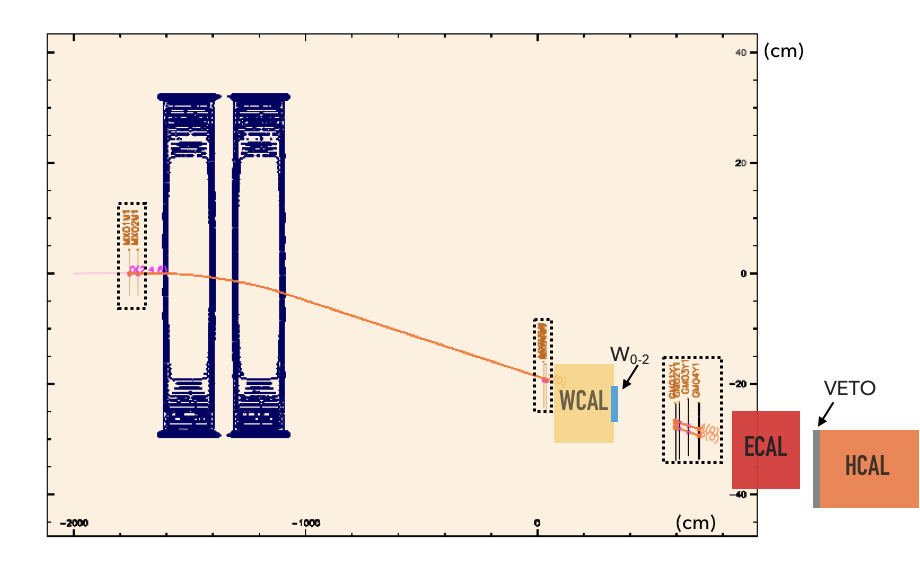
\includegraphics[width=\textwidth]{thesis_figures/MC_reco/CORAL_display_2.png}
 \caption{Track reconstruction display from CORAL.}
 \label{fig:CORAL_display}
 \end{figure}

\subsection{Momentum Reconstruction}
\label{subsec:mom_reco}
The momentum reconstruction in CORAL was checked by selecting the reconstructed tracks which were bridged through the magnets successfully. It was made sure that all tracking detectors upstream and downstream that are involved in momentum reconstruction had a contribution to the track i.e each detector had a hit which was used to reconstruct the final fitted track. In our case this meant the four Micromega detectors.
 \begin{figure}[h!]
 \centering
 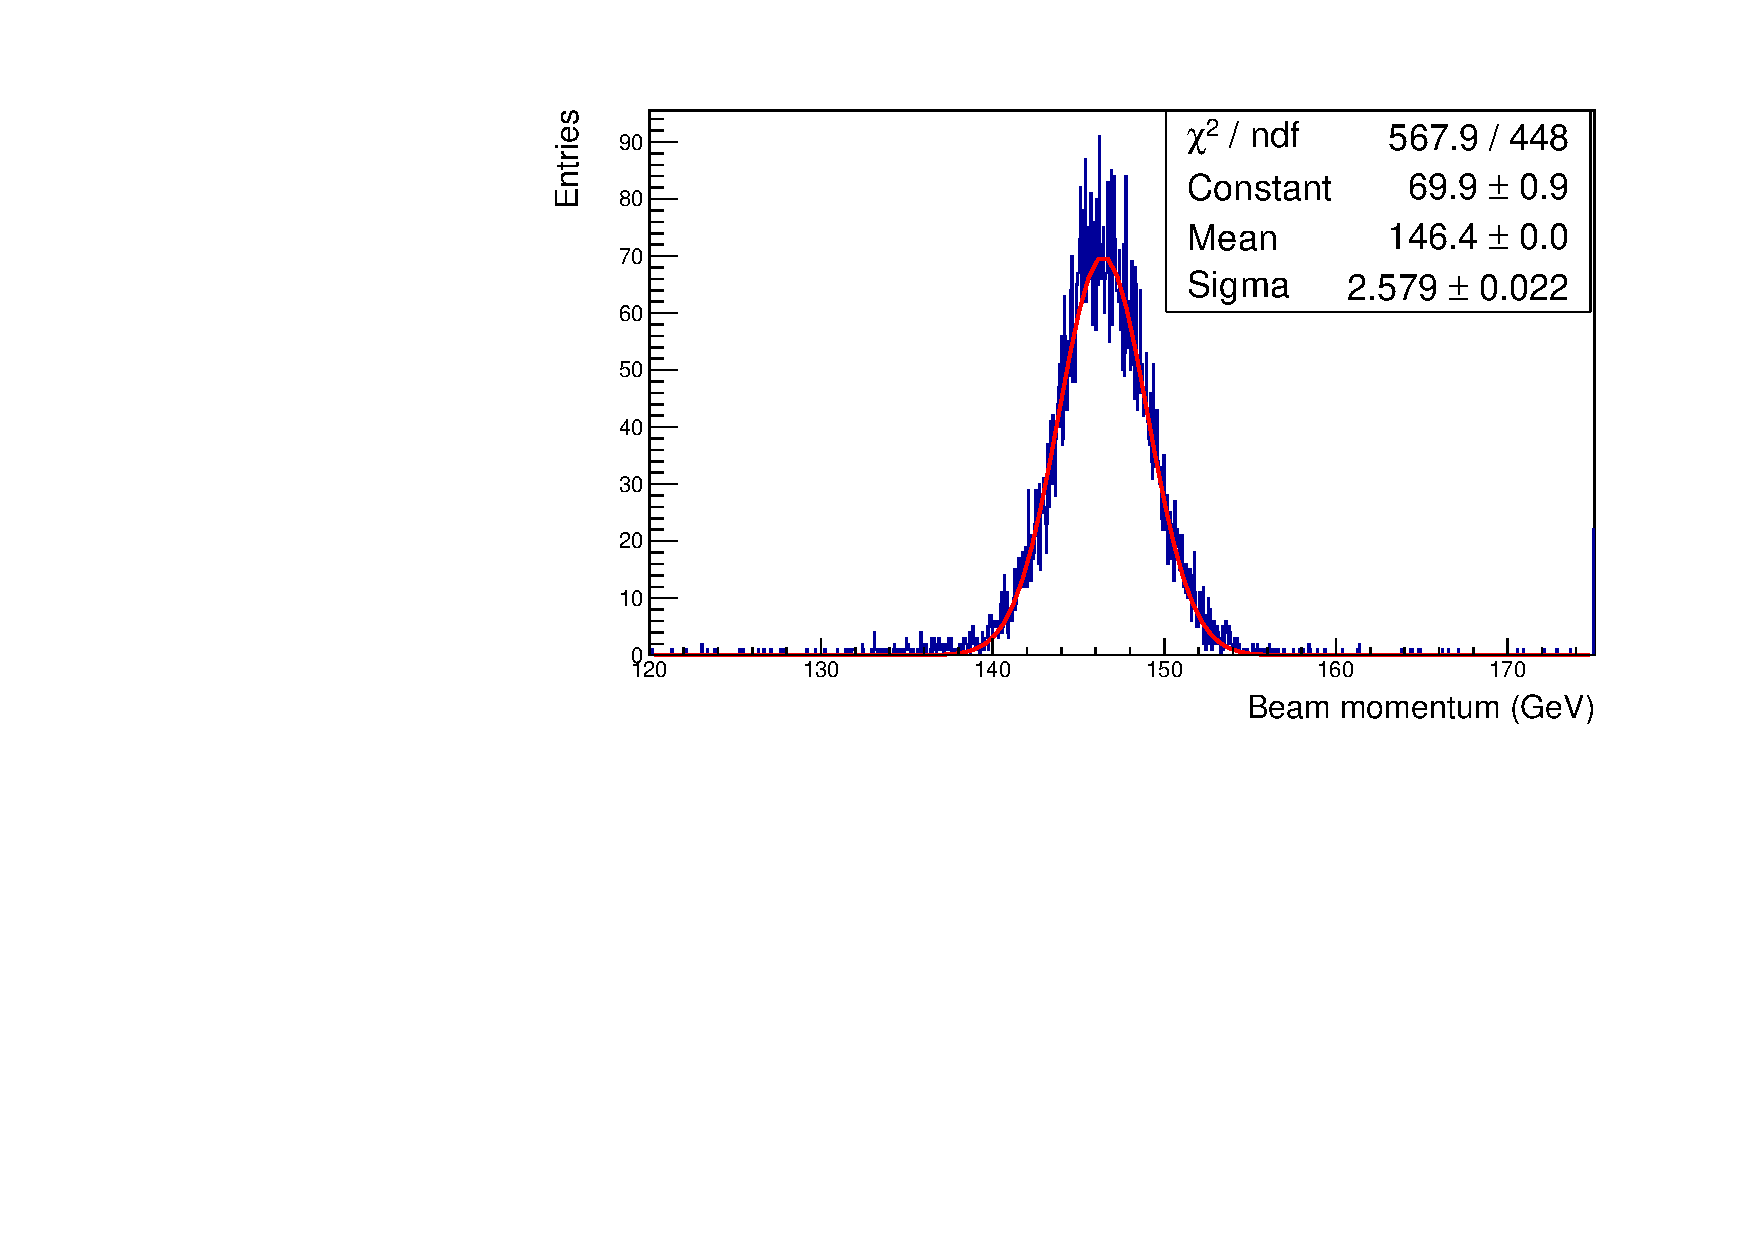
\includegraphics[width=0.9\textwidth]{thesis_figures/MC_reco/beam_mom_bigger_axis.pdf}
 \caption{Reconstructed beam momentum in CORAL along with fit parameters.}
 \label{fig:reco_beam_mom}
 \end{figure}

Fig.(\ref{fig:reco_beam_mom}) shows the reconstructed beam momentum. The momentum was fitted with a standard Gaussian function. The extracted momentum after reconstruction has a value of $146.4 ~\text{GeV}$ with an error of $2.58 ~\text{GeV}$. Even though we have a beam which has a momentum of $150 ~\text{GeV}$ after simulation, we observe that the reconstructed beam momentum is much lower. Since the detectors in the reconstruction were placed at the exact position as that of the simulation, the reason for the observed beam momentum distribution can be either attributed to the difference in the integrated magnetic field between the simulation and the reconstruction or it can also be due to some systematic error of the track reconstruction and momentum determination algorithm. The Gaussian spread in the reconstructed momentum should be due to the resolution of the detectors mimicked in the reconstruction.

The magnetic field in the simulation is implemented as a box field with an integrated field strength of $7.85~\text{Tm}$ while in the reconstruction the measured field maps of the magnets made for the physics runs are used. Even though the integrated magnetic fields for both the implementations are almost the same the bending effect which might be present due to the fringe fields is only simulated during the reconstruction. This might be the reasons for the the underestimation of the calculated beam momentum compared to the one simulated.

To check the performance of the tracking algorithm for momentum reconstruction the angles of the incoming track were compared to the fitted momentum after track fitting. Figures (\ref{fig:reco_mom_dip}) and (\ref{fig:reco_mom_azi}) show the obtained result. Both of the angles are chosen from the fitted track piece which is upstream of the magnet. The dip angle is defined as the angle of the track which moves it in a plane parallel to the magnetic field lines hence during the bending process this angle is not affected and does not contribute to the momentum reconstruction. As seen in the fig.(\ref{fig:reco_mom_dip}) the fitted momentum over the distribution of the dip angle is uniform which is as expected.

The azimuthal angle is the angle of the track piece which moves it in a direction perpendicular to that of the magnetic field. This is the angle affected by the bending field of the magnet and is critical for momentum reconstruction. As we see in fig.(\ref{fig:reco_mom_azi}) there is a correlation between the fitted momentum and the incoming track's azimuthal angle. This shows that during the reconstruction, tracks with varying azimuthal angles were reconstructed which led to a spread in the reconstructed beam momentum. This might add some systematic uncertainties to the beam momentum observed and should be investigated further examining the reconstruction algorithm in CORAL in future studies.

 \begin{figure}[t!]
 \centering
 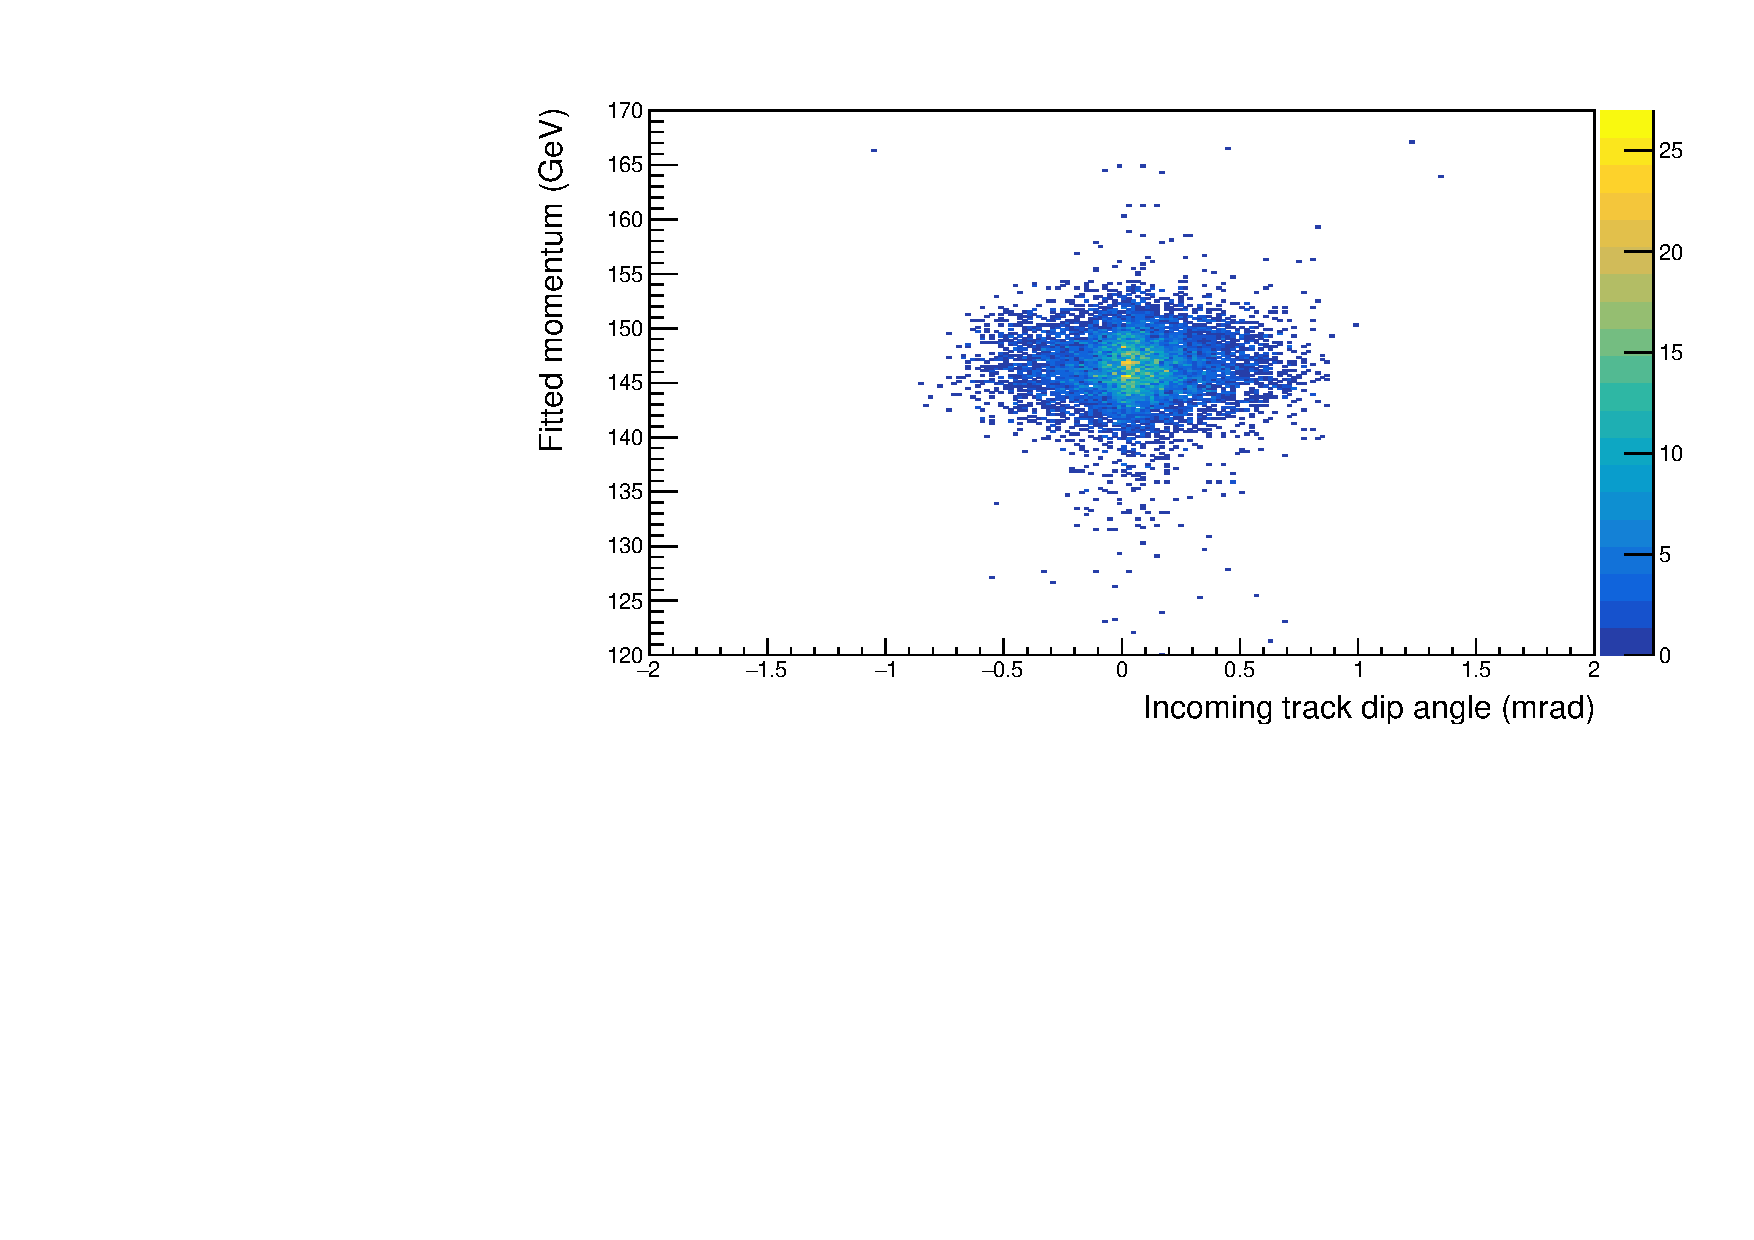
\includegraphics[width=\textwidth]{thesis_figures/MC_reco/mom_vs_dip.pdf}
 \caption{Fitted beam momentum vs dip angle of incoming track. }
 \label{fig:reco_mom_dip}
 \end{figure}

 \begin{figure}[h!]
 \centering
 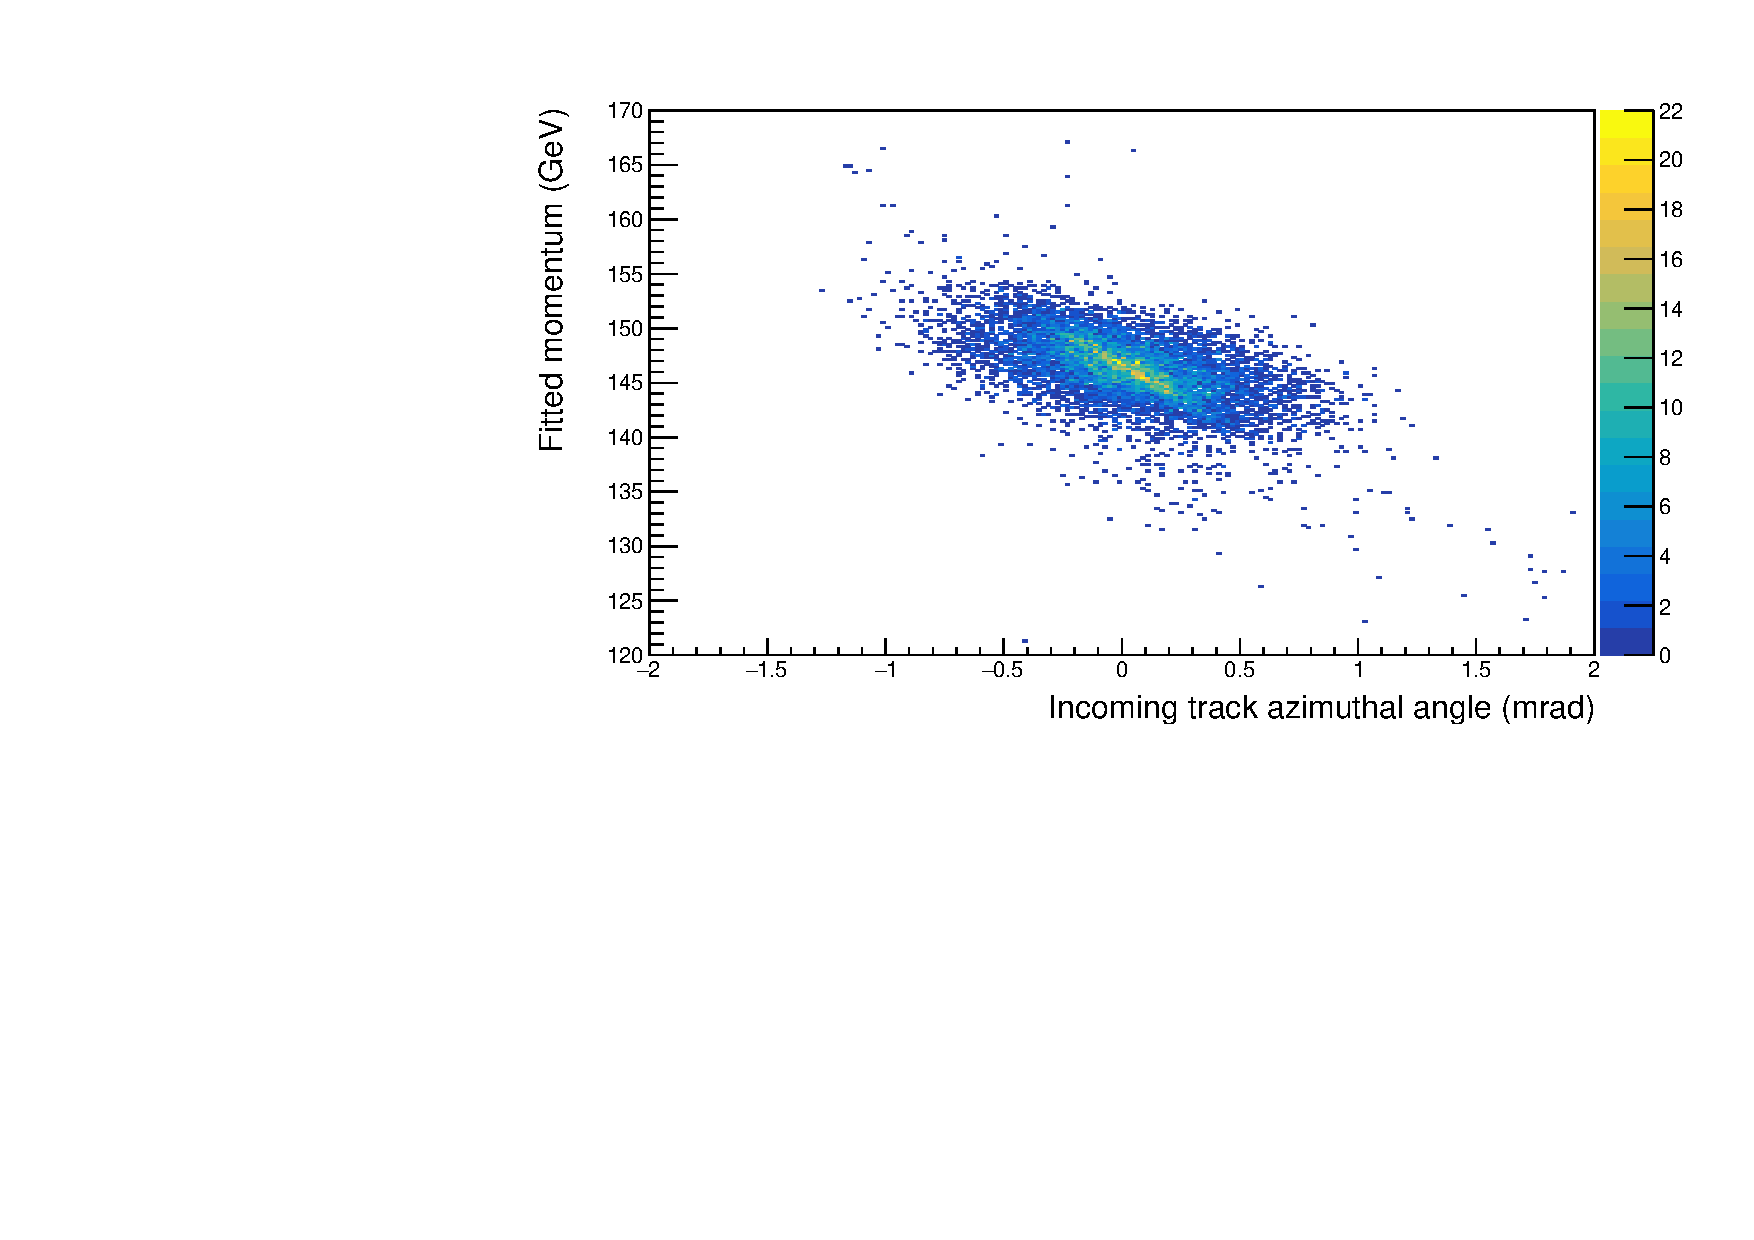
\includegraphics[width=\textwidth]{thesis_figures/MC_reco/mom_vs_azi.pdf}
 \caption{Fitted beam momentum vs azimuthal angle of incoming track.}
 \label{fig:reco_mom_azi}
 \end{figure}
\newpage

 \subsection{A' Reconstruction}
 \label{subsec:a'_reco}
The $A'$ reconstruction in CORAL was looked at in two stages. The first included identifying the $A'$ events in the reconstructed sample and the second included studying the decay products of the $A'$ which are the $e^+ e^-$.

The $A'$ events were selected by applying the following cuts:
\begin{enumerate}
  \item $142~\text{GeV} < E_{WCAL} < 150~\text{GeV} $.
  \item $E_{W_{0-2}}, E_{ECAL} > 0~\text{GeV}$.
  \item Two tracks in downstream GEM detectors.
  \item $E_{VETO} = E_{HCAL} = 0~\text{GeV} $.
\end{enumerate}

These cuts helped separate the $A'$ events from the rare dimuon events mentioned before. The angular distribution of the two track events were analyzed and is shown in fig.(\ref{fig:reco_angle}). The figure shows that most of the $e^+ e^-$ pairs produced from the decay of $A'$ have a small outgoing angle. This is as expected since we assume that the $A'$ which might be produced in a real physics event might be highly boosted in the forward direction which will result in a smaller opening angle for the decay products. The current expected limit for this opening angle for $1 \lesssim m_{A'}\lesssim 25 \text{MeV}$ at $E_{A'}=$20~GeV is $\theta \ll 2\text{mrad}$ as mentioned in~\cite{Banerjee_2018}. This also validates our reasoning to not implement shower clusterization in the downstream calorimeters since at such small angles, with the current size of our individual calorimeter cell, the shower will not achieve the necessary separation required for identifying individual particles.
\FloatBarrier
%\clearpage
 \begin{figure}[t!]
 \centering
 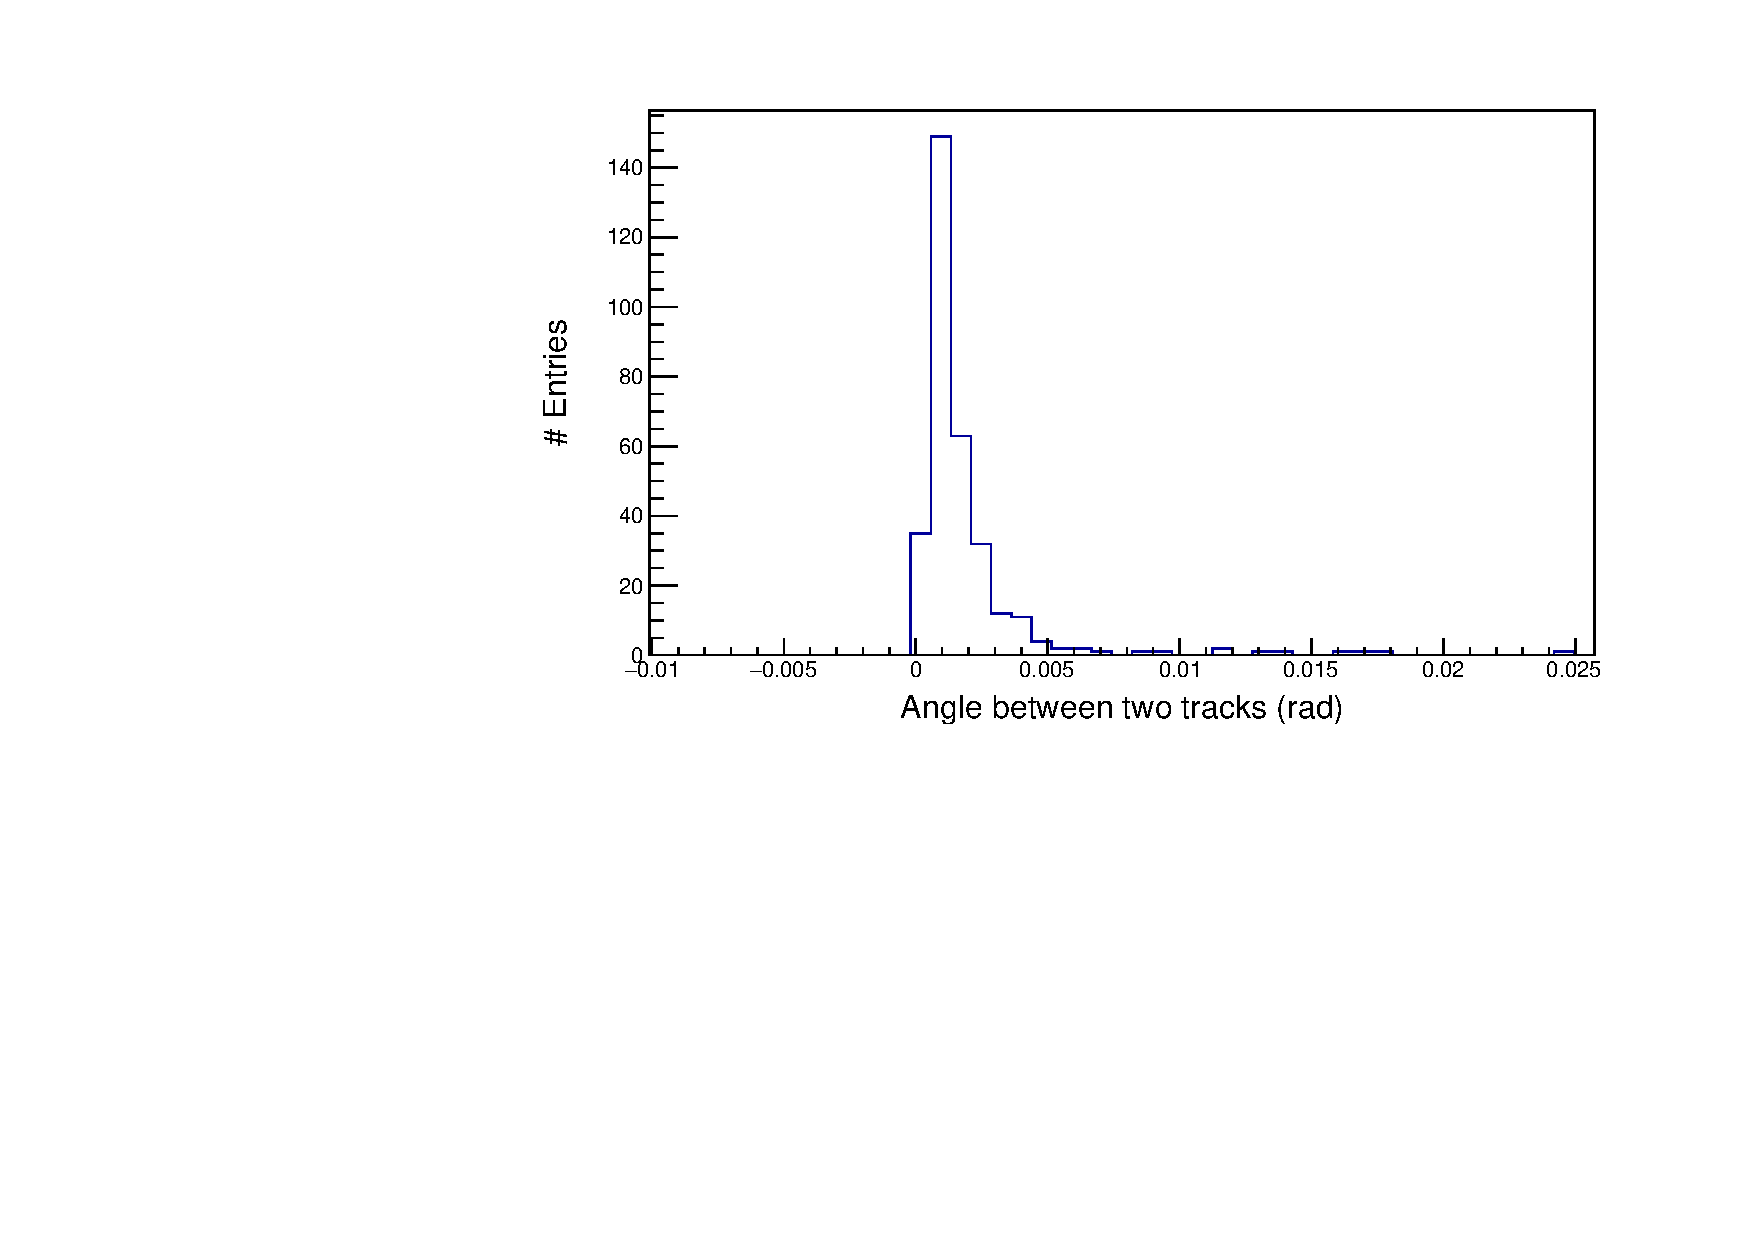
\includegraphics[width=\textwidth]{thesis_figures/MC_reco/ang_dist_final.pdf}
 \caption{Angle between the outgoing $e^+e^-$ tracks}
 \label{fig:reco_angle}
 \end{figure}


%%% Local Variables:
%%% mode: latex
%%% TeX-master: "mythesis"
%%% End:
